%=== tipo di documento ================================================================
\documentclass[a4paper]{report}
%=== pacchetti da usare ===============================================================
\usepackage[T1]{fontenc} % codifica dei font per l'italiano
\usepackage[utf8]{inputenc} % lettere accentate da tastiera
\usepackage[italian]{babel} % lingua del documento
\usepackage[shortlabels]{enumitem}%per fare elenchi ad hoc
\usepackage{framed}% per riquadrare il testo
\usepackage{amsmath}% per avere le formule matematiche fatte bene
\usepackage{amssymb}% per avere le formule matematiche fatte bene
\usepackage{amsthm}%per fare i teoremi in modo ordinato
\usepackage[big]{layaureo} %per avere i margini più stretti
\usepackage{graphicx} %per inserire le immagini
\usepackage{mathtools}
\usepackage{mathabx}
\usepackage{cancel}
%=== lettere speciali =================================================================
\makeatletter
\newcommand{\superimpose}[2]{%
  {\ooalign{$#1\@firstoftwo#2$\cr\hfil$#1\@secondoftwo#2$\hfil\cr}}}
\makeatother
\def\retro{\ensuremath{%
  \reflectbox{\rotatebox[origin=c]{180}{$\circlearrowleft$}}}}
\newcommand{\R}{\mathbb{R}}%reali
\newcommand{\retroneg}{\mathpalette\superimpose{{\retro}{-}}} %retroazione negativa
\DeclareMathOperator{\tr}{tr} %traccia
\newcommand{\parallelsum}{\mathbin{\|}}%parallelo
%==== imposto la directory delle immagin i ============================================
\graphicspath{ {./images/} }
%==== documento =======================================================================
\begin{document}
%=== titolo e sottotitolo =============================================================
\begin{center}
\section*{Fondamenti di Automatica}
\section*{Simulazione 2}
L. Maci, L. Paparo, M. Poggi, J. Stringara e G. Venturini
\end{center}
%=== quesito 1 ========================================================================
\subsection*{Quesito 1}
Si consideri la rete idrica in figura composta da due serbatoi collegati in cascata caratterizzati dai
volumi di invaso $x_1$ e $x_2$ e dalle costanti di deflusso $k_1 = 6$ e $k_2 = 1$. Il primo serbatoio è alimentato da
una portata di ingresso u mentre sul secondo agisce un disturbo $d$.
%=== figura ===========================================================================
\begin{figure}[h]

\includegraphics[width=\textwidth]{sysgraf}
\end{figure}\newline
%======================================================================================
Volendo fare in modo che la portata di uscita dal
secondo serbatoio $y$ sia più possibile prossima
a una portata  desiderata  $\overline{w}$  
occorre  compensare  l’effetto  del  disturbo  $d$
sull’uscita $y$  supponendo  che  la  variabile di 
ingresso $u$ segua la legge:
%=== equazione ingresso nuovo =========================================================
\[
  u=\overline{w}-\alpha(y-\overline{w})\quad \quad \quad \alpha >0
\]
%=== punto a) =========================================================================
\subsubsection*{Punto a:}
%=== equazioni del sistema ============================================================
In primo luogo scriviamo le equazioni del sistema:
\begin{align*}
\dot{x}_1&=u-k_1x_1\\
\dot{x}_2&=k_1x_1-k_2x_2+d\\
y&=k_2x_2\\
\end{align*}
%=== sistema con nuovo ingresso =======================================================
Ora consideriamo il nuovo ingresso $u=\overline{w}-\alpha (y-\overline{w})$
\begin{align*}
\dot{x}_1&=(1+\alpha)\overline{w}-\alpha k_2x_2-k_1x_1\\
\dot{x}_2&=k_1x_1-k_2x_2+d\\
y&=k_2x_2
\end{align*}
%=== punto b ==========================================================================
\subsubsection*{Punto b:}
%=== matrice di sistema ===============================================================
Ciò significa che la matrice A sarà:
\[
A=\begin{bmatrix}
-k_1 & -\alpha k_2\\
k_1 & -k_2
\end{bmatrix}
\]
%=== sistema traccia e determinante ===================================================
Per capirne la stabilità usiamo il criterio di traccia e determinante:
\[
\left\{\begin{array}{l}
tr(A)=-k_1-k_2<0 \longrightarrow \text{ che è vero }\forall \alpha\\
\det(A)=k_1k_2(1+\alpha)>0\longrightarrow \alpha>-1
\end{array}\right.
\]
%======================================================================================
Dunque il sistema sarà sempre \textbf{Asintoticamente Stabile} poichè la traccia del problema ci dice che $\alpha >0$ per ipotesi (e ciò include l'insieme $\alpha > -1$). \newline
Ora supponendo $d$ costante all'equilibrio avremo le equazioni:
%=== equazioni all'equilibrio =========================================================
\begin{align*}
0&=(1+\alpha)\overline{w}-\alpha k_2x_2-k_2x_1\\
0&=k_1x_1-k_2x_2+d\\
y&=k_2x_2
\end{align*}
%=== variabili all'equilibrio =========================================================
Che se rilavorate ci danno:
\begin{align*}
\overline{x}_1&=\frac{1}{k_1}\left(\overline{w}-\frac{\alpha d}{(1+\alpha)}\right)\\
\overline{x}_2&=\frac{1}{k_2}\left(\overline{w}+\frac{d}{(1+\alpha)}\right)\\
\overline{y}&=\overline{w}+\frac{d}{(1+\alpha)}
\end{align*}
%=== autovalori della matrice A  e tempi di riposta ===================================
Ora scopriamo gli autovalori della matrice A scrivendoci il polinomio caratteristico usando traccia e determinante:
\[
\lambda^2-tr(A)\lambda+\det(A)=\lambda^2+(k_1+k_2)\lambda+k_1k_2(1+\alpha)\overset{k_1=6, k_2=1}{\longrightarrow}\lambda^2+7\lambda+6(1+\alpha)
\]
Che ci dà i valori:
\[
\lambda_{1,2}=\frac{-7\pm\sqrt{25-24\alpha}}{2}
\]
Dunque:
\begin{align*}
&\text{Se } \alpha \geq\frac{25}{24} \quad \Re(\lambda_{1,2})=-\frac{7}{2}\\
&\text{In caso contrario } -\frac{7}{2}<\Re(\lambda_D)<-1
\end{align*}
%=== grafico tempo di risposta ========================================================
Dandoci il seguente grafico per il tempo di risposta $T_R$ del sistema:
\begin{center}
\begin{figure}[h]
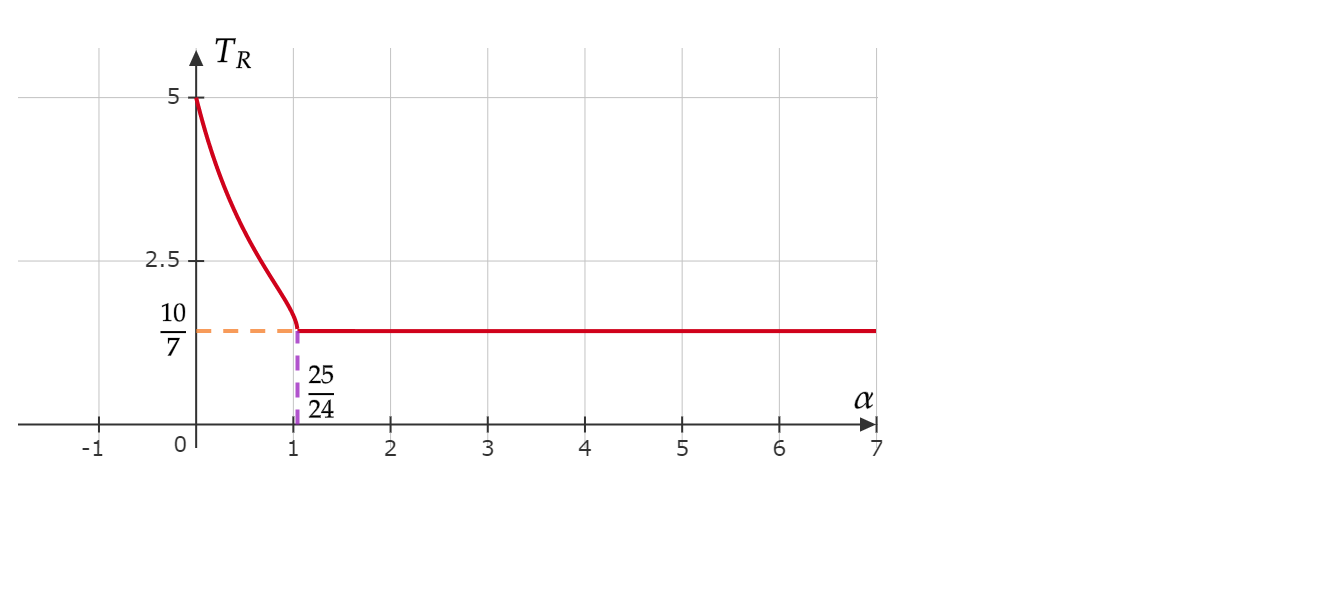
\includegraphics[width=\textwidth]{diagtd}
\end{figure}
\end{center}
\newpage
%=== punto c ==========================================================================
\subsubsection*{Punto c:}
%=== dati da usare ====================================================================
Dati $\overline{w}=10,\alpha=2$ e:
\[
d=\left\{\begin{array}{l}
3 \text{ per } 0\leq t \leq 5\\
0 \text{ altrimenti}
\end{array}
\right.
\]
Avremo le seguenti situazioni:
\bigskip \newline
%=== caso 0<t<5 ===============================================================================
\boxed{0\leq t\leq 5} 
\medskip\newline
Ora nel caso $0\leq t\leq5$ le equazioni di equilibrio diventano:
%=== equilibrio per 0<t<5 =====================================================================
\begin{align*}
\overline{x}_1&=\frac{1}{k_1}\left(\overline{w}-\frac{\alpha d}{(1+\alpha)}\right)\longrightarrow\frac{1}{6}\left(10-\frac{2\cdot 3}{1+2}\right)=\frac{4}{3}\\
\overline{x}_2&=\frac{1}{k_2}\left(\overline{w}+\frac{d}{(1+\alpha)}\right)\longrightarrow\frac{1}{1}\left(10+\frac{3}{1+2}\right)=11\\
\end{align*}
%=== giustificazione traiettoria ==============================================================
Ora poichè siamo nel caso di autovalori complessi il sistema sarà asintoticamente stabile e convergerà all'equilibrio come ad un \textbf{Fuoco Stabile} dunque seguirà una spirale verso l'equilibrio $\left(\frac{4}{3},11\right)$, cerchiamo ora il verso di questa spirale:
%=== lungo gli assi le derivate sono ==========================================================
\[
x_1=\frac{4}{3}\implies\left\{\begin{array}{l}
\dot{x}_1=22-2x_2 \\
\dot{x}_2=11-x_2
\end{array}
\right.\text{ che per }x_2<11 \text{ ci danno: } \left\{\begin{array}{l}
\dot{x}_1>0\\
\dot{x}_2>0
\end{array}\right.
\]
%=== traiettoria per d=3 ======================================================================
Dunque il senso della spirale sarà \textbf{anti-orario} e il grafico sarà circa il seguente:
\begin{figure}[h]
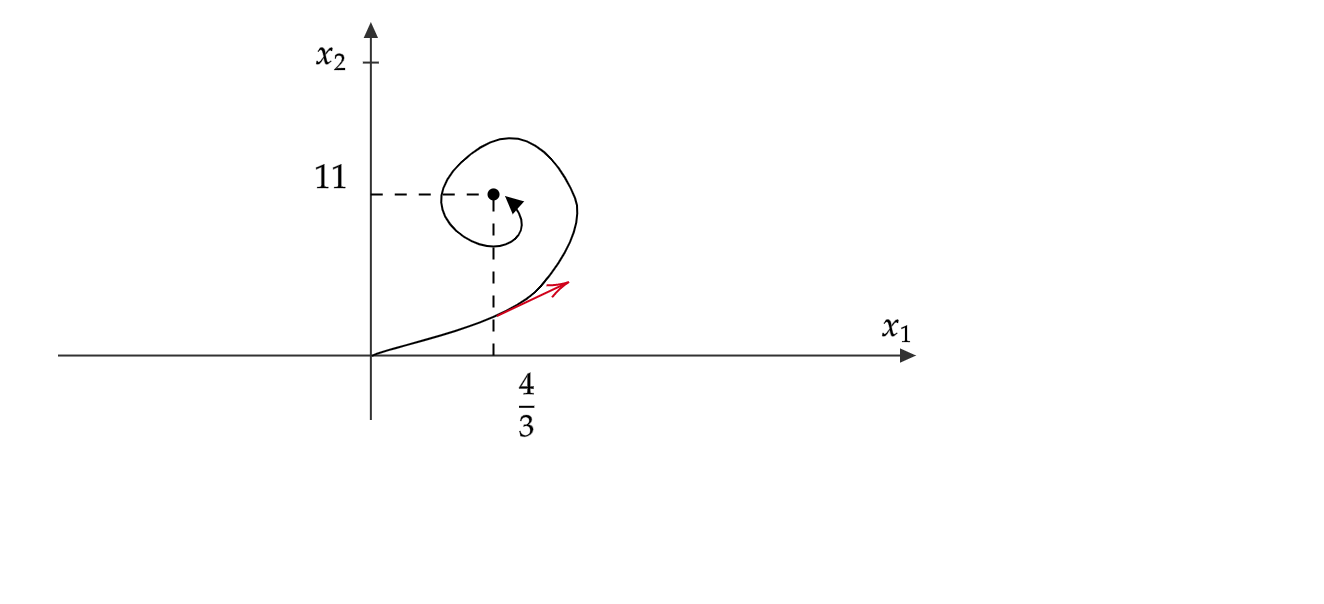
\includegraphics[width=\textwidth]{diagtj1}
\end{figure}\newline
Inoltre notiamo che quest'equilibrio verrà raggiunto già in questo intervallo poichè $T_R<5$.
 \bigskip\newline
%=== t>5 =====================================================================================
\boxed{t>5} 
\medskip\newline
Similmente per $t>5$ avremo un nuovo equilibrio:
%=== equilibrio per 0<t<5 =====================================================================
\begin{align*}
\overline{x}_1&=\frac{1}{k_1}\left(\overline{w}-\frac{\alpha d}{(1+\alpha)}\right)\longrightarrow\frac{1}{6}\left(10-\frac{2\cdot 0}{1+2}\right)=\frac{5}{3}\\
\overline{x}_2&=\frac{1}{k_2}\left(\overline{w}+\frac{d}{(1+\alpha)}\right)\longrightarrow\frac{1}{1}\left(10+\frac{0}{1+2}\right)=10\\
\end{align*}\newpage
Poichè gli autovalori rimangono invariati avremo un altro \textbf{Fuoco Stabile} che partendo da $\left(\frac{4}{3},11\right)$ si avvita su $\left(\frac{5}{3},10\right)$ e similmente a come abbiamo svolto per $0\leq t\leq 5$ troviamo che la spirale ha sempre verso \textbf{anti-orario}, e quindi avrà circa questo andamento:
%=== diagramma traiettorie 2 ==================================================================
\begin{figure}[h]
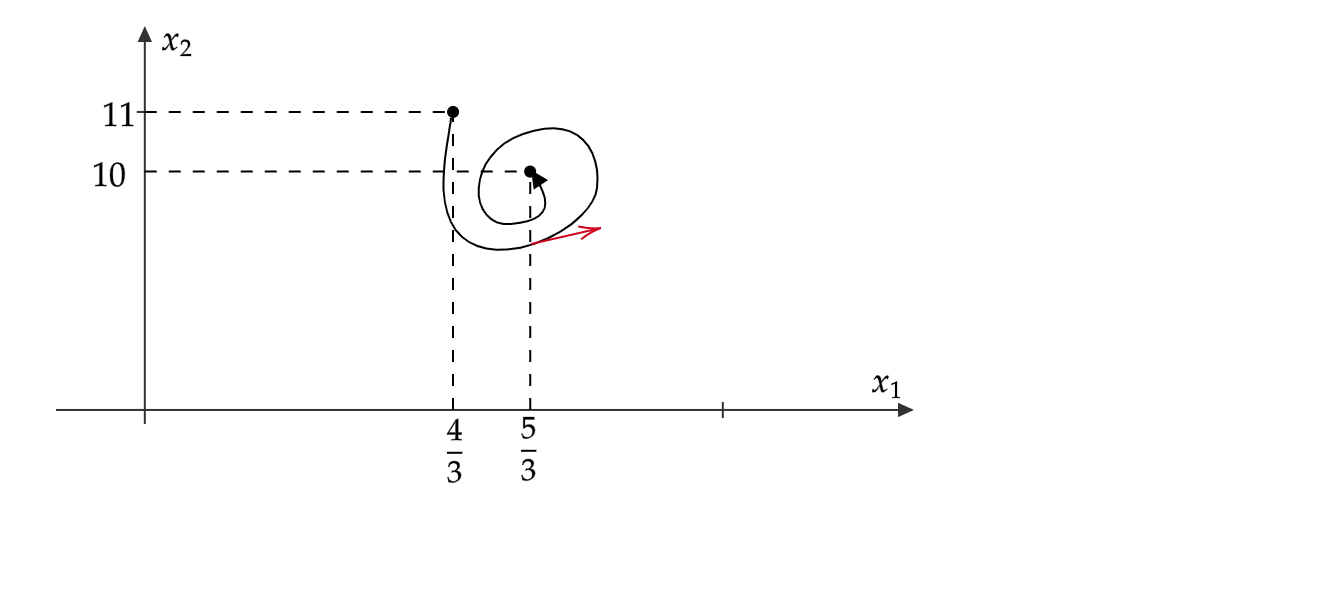
\includegraphics[width=\textwidth]{diagtj2}
\end{figure}
%=== domanda 2 ================================================================================
\subsection*{Quesito 2}
Si consideri il seguente sistema non lineare a tempo continuo del second’ordine:
\begin{align*}
\dot{x}_1&=3x_1+4x_2-x_2^2-4\\
\dot{x}_2&=x_1-3
\end{align*}
%=== punto a =================================================================================
\subsubsection*{Punto a:}
%=== linearizzazione del problema =============================================================
Partiamo linearizzando il problema, per fare ciò scriviamoci la \textbf{matrice Jacobiana} del sistema:
\[
J(x)=\begin{bmatrix}
3 & 4-2x_2\\
1 & 0
\end{bmatrix}
\]
%=== punti con derivata nulla =================================================================
Ora cerchiamo i punti che annullano le derivate del sistema:
\[
\left\{\begin{array}{l}
0=3x_1+4x_2-x_2^2-4\\
0=x_1-3
\end{array}
\right.\implies\left\{\begin{array}{l}
x_2=5 \lor x_2=-1\\
x_1=3
\end{array}
\right.
\]
Quindi abbiamo il punto $p_1=\left(\begin{array}{c}
3\\
5
\end{array}\right)$ e il punto $p_2=\left(\begin{array}{r}
3\\
-1
\end{array}\right)$, ora valutiamo $J(x)$ in $p_1$ e $p_2$:
\[
J(p_1)=\begin{bmatrix}
3 & -6\\
1 & 0
\end{bmatrix} \quad J(p_2)=\begin{bmatrix}
3 & 6\\
1 & 0
\end{bmatrix}
\]
%=== autovalori punti di equilibrio ===================================================
E usando  traccia e determinante troviamo i seguenti polinomi caratteristici:
\begin{align*}
&J(p_1)\longrightarrow \lambda^2-3\lambda+6\longrightarrow \lambda_{1,2}=\frac{3\pm\sqrt{9-24}}{2}\longrightarrow \lambda_{1,2}\in\mathbb{C} \text{ e }\Re(\lambda_{1,2})=\frac{3}{2}\\
&J(p_2)\longrightarrow \lambda^2-3\lambda-6\longrightarrow \lambda_{1,2}=\frac{3\pm\sqrt{9+24}}{2}\longrightarrow \lambda_{1,2}\in\R \text{ e } \lambda_1<0 \text{ e } \lambda_2>0
\end{align*}
Perciò in $p_1$ avremo una situazione di \textbf{Fuoco Instabile} e in $p_2$ una \textbf{Sella}.\newpage
%=== punto b ==========================================================================
\subsubsection*{Punto b:}
%=== fuoco stabile ====================================================================
Come abbiamo accennato sopra il punto $p_1$ è un \textbf{Fuoco Instabile}, come svolto nel quesito 2 per valutarne il verso studiamo la derivata in un suo intorno e troviamo un grafico simile:
\begin{figure}[h]
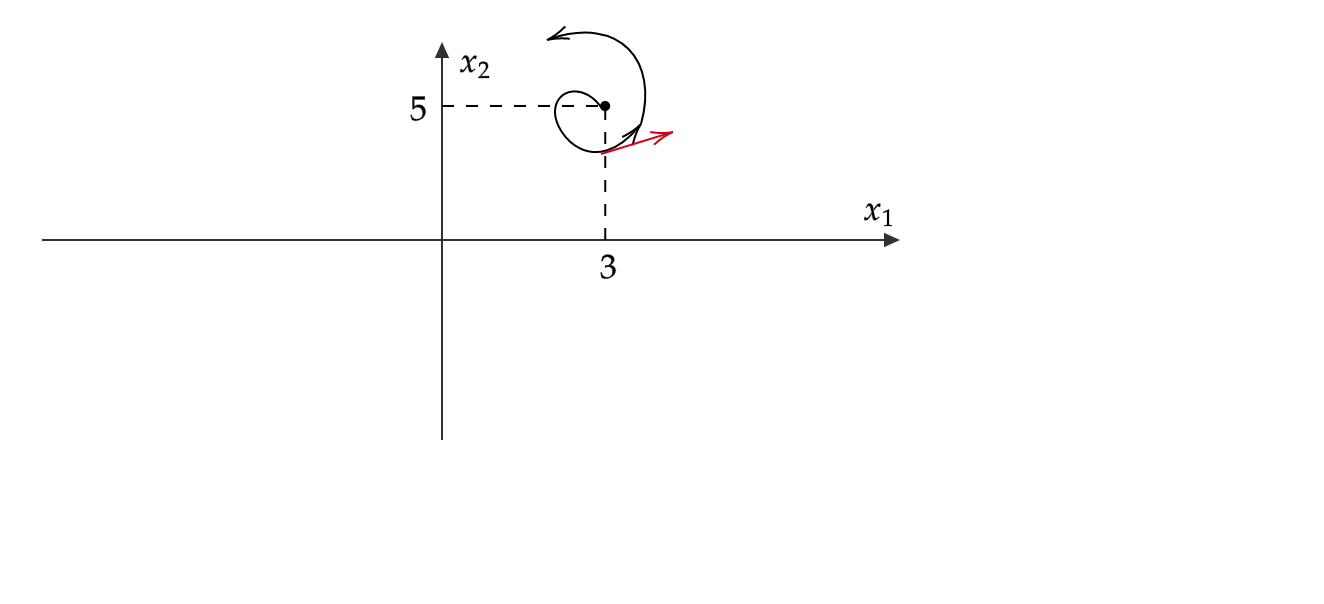
\includegraphics[width=\textwidth]{eqp1}
\end{figure}\newline
%=== sella ============================================================================
Per il punto $p_2$ invece abbiamo una situazione di \textbf{Sella}, per capire il verso delle derivate cerchiamo gli autovettori della matrice Jacobiana in $p_2$:
%=== autovalori ed autovettori jacobiana ==============================================
\begin{align*}
&\lambda_1=\frac{3+\sqrt{33}}{2}\longrightarrow J(p_2)w=\lambda_1 w\longrightarrow w_2=\frac{2}{3+\sqrt{33}} w_1\\
&\lambda_2=\frac{3-\sqrt{33}}{2}\longrightarrow J(p_2)w=\lambda_2 w\longrightarrow w_2=\frac{2}{3-\sqrt{33}} w_1
\end{align*}
%=== grafico punto di sella ===========================================================
Che quindi ci danno il seguente grafico approssimativo:
\begin{figure}[h]
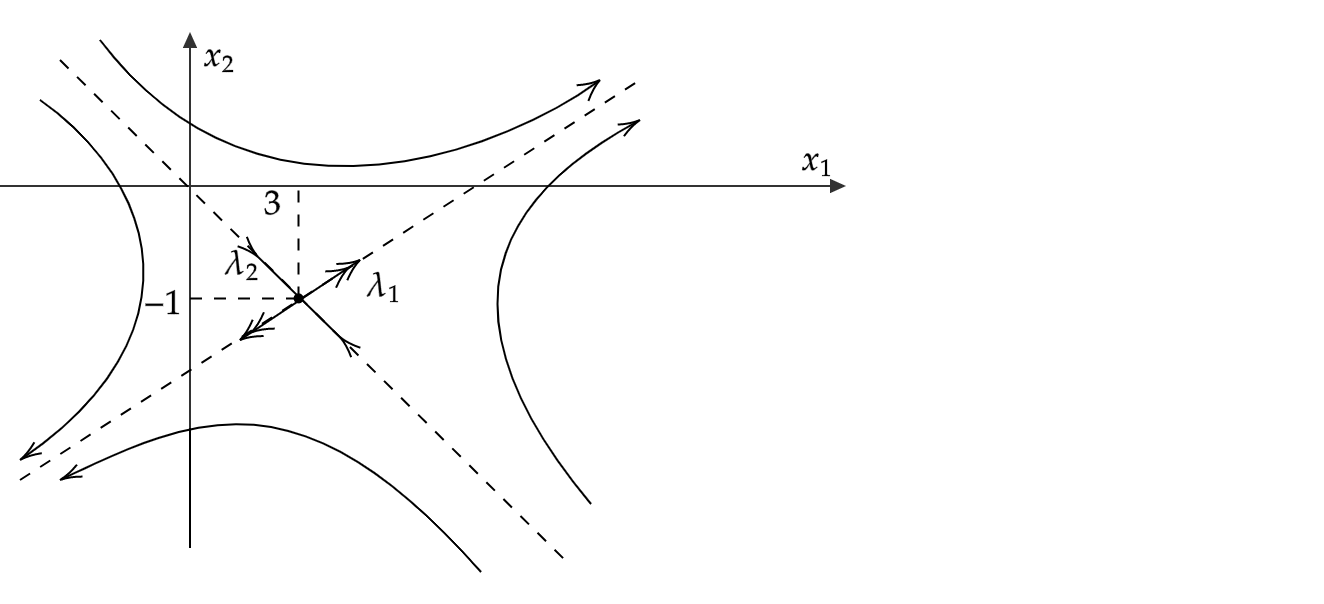
\includegraphics[width=\textwidth]{eqp2}
\end{figure}
%=== punto c ==========================================================================
\subsubsection*{Punto c:}
Per studiare la direzione del vettore tangente alle traiettorie dobbiamo prima scrivere le isocline. Notiamo che:
\[
\dot{x}_2>0\implies x_1>3 \text{ e } \dot{x}_1>0\implies x_1>\frac{1}{3}(x_2^2-4x_2+4)
\]\newpage
Che ci porta a scrivere il seguente grafico:
\begin{figure}[h]
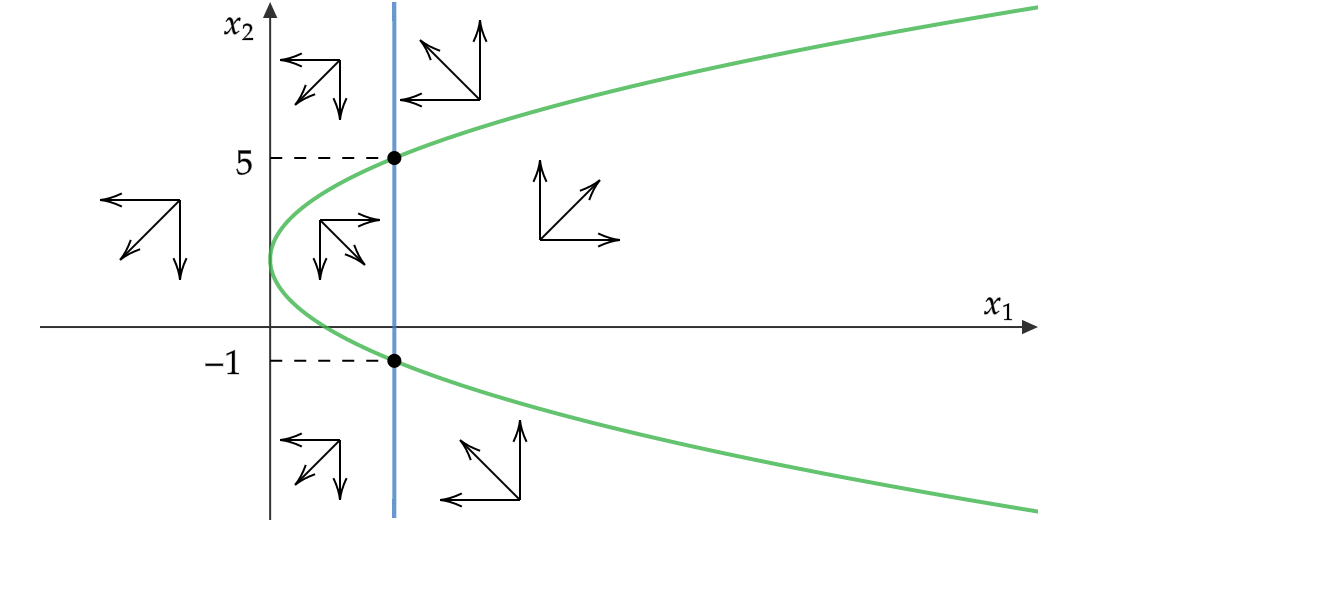
\includegraphics[width=\textwidth]{isocline}
\end{figure}
%=== punto d ==========================================================================
\subsubsection*{Punto d:}
Per disegnare l'ultimo grafico non ci resta che unire tutto insieme:
\begin{figure}[h]
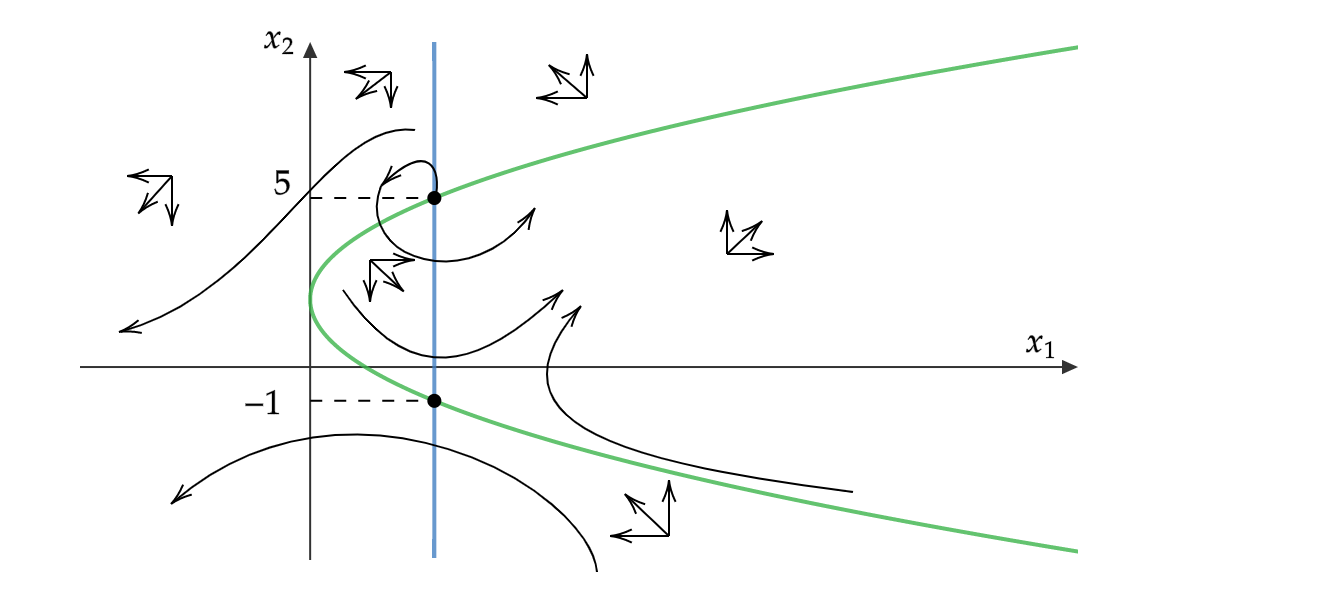
\includegraphics[width=\textwidth]{trajectories}
\end{figure}
%=== domanda 3 ========================================================================
\subsection*{Quesito 3}
Si consideri il seguente sistema lineare a tempo continuo:
\begin{align*}
\dot{x}_1&=2x_1-6x_2\\
\dot{x}_2&=x_1-x_2+u\\
y&=x_2
\end{align*}
%=== punto a ==========================================================================
\subsubsection*{Punto a:}
%=== variabili di sistema =============================================================
In primis scriviamoci le variabili di sistema
\begin{align*}
A=\begin{bmatrix}
2 & -6\\
1 & -1
\end{bmatrix} b=\begin{bmatrix}
0\\ 1
\end{bmatrix}\\
c=\begin{bmatrix}
0 & 1
\end{bmatrix} \quad \quad d=0
\end{align*}
%=== stabilità ========================================================================
Per studiare la stabilità analizziamo la matrice $A$. Notiamo subito che $tr(A)=1>0$ e $\det(A)=4>0$ dunque per il criterio di traccia e determinante il sistema è \textbf{Instabile}. Per capire invece  se ammetta o meno un \textbf{Regolatore Asintotico} studiamo la sua matrice di osservabilità e di raggiungibilità:
\begin{align*}
O=\begin{bmatrix}
c\\
cA
\end{bmatrix}\longrightarrow\begin{bmatrix}
0 & 1 \\
2 & -1
\end{bmatrix}\\
R=\begin{bmatrix}
b && Ab
\end{bmatrix}\longrightarrow\begin{bmatrix}
0 & -6 \\
1 & -1
\end{bmatrix}
\end{align*}
%=== osservabilità e raggiungibilità ==================================================
Che hanno entrambe determinante diverso da zero, il sistema è \textbf{Completamente Osservabile}  e \textbf{Completamente Raggiungibile}, perciò ammetterà un \textbf{Regolatore Lineare} e si potranno scegliere a piacere gli autovalori del sistema regolato.
%=== punto b ==========================================================================
\subsubsection*{Punto b:}
Poichè il tempo di risposta $T_R$ cercato è 5 ciò ci dice che il tempo dominante del sistema dovrà essere 1 e che dunque poichè $T_D=-\frac{1}{\Re(\lambda_D)}$ che $\Re(\lambda_D)=-1$. Per comodità scegliamo \textbf{tutti} gli autovalori di $A+bk$ uguali a $-1$. Inoltre poichè l'errore di stima dello stato deve tendere a $0$ in 1 unità di tempo l'autovalore dominante di $A+lc$ dovà invece essere -5, come sopra scegliamo anche l'altro autovalore uguale a -5. Si noti che dato che gli autovalori del sistema regolato sono l'unione di quelli di $A+bk$ e di $A+lc$ la scelta appena operata non va ad influenzare il tempo di risposta del sistema regolato. \newline
Ora cerchiamo i valori di $l$ e $k$ tali da rendere questa condizione veritiera. Partiamo da $k$:
%=== vettore k ========================================================================
\[
A+bk=\begin{bmatrix}
2 & -6\\
1 & -1
\end{bmatrix} + \begin{bmatrix}
0\\ 1
\end{bmatrix} \begin{bmatrix}
k_1 & k_2
\end{bmatrix}= \begin{bmatrix}
2 & -6\\
1+k_1 & -1+k_2
\end{bmatrix}
\]
Tramite traccia e determinante ci costruiamo questo sistema:
\[
\left\{\begin{array}{l}
1+k_2=-2\\
2(-1+k_2)+6(1+k_1)=1
\end{array}\right.\longrightarrow k=\begin{bmatrix}
\frac{1}{2} & -3
\end{bmatrix}
\]
%=== vettore l ========================================================================
Svolgiamo lo stesso per $O$:
\[
A+bk=\begin{bmatrix}
2 & -6\\
1 & -1
\end{bmatrix} + \begin{bmatrix}
l_1 \\ l_2
\end{bmatrix} \begin{bmatrix}
0 & 1
\end{bmatrix}= \begin{bmatrix}
2 & -6+l_1\\
1 & -1+l_2
\end{bmatrix}
\]
Come sopra ricaviamo:
\[
\left\{\begin{array}{l}
1+l_2=-10\\
2(-1+l_2)-(-6+l_1)=25
\end{array}\right.\longrightarrow l=\begin{bmatrix}
-43\\
-11
\end{bmatrix}
\]
%=== punto c ==========================================================================
\subsubsection*{Punto c:}
Aggiungere una retroazione statica significa sostituire sostituire ad $u$ un certo $\alpha y$ con $\alpha\in\R$, e dunque il sistema diventa:
\begin{align*}
\dot{x}_1&=2x_1-6x_2\\
\dot{x}_2&=x_1-x_2+\alpha x_2
\end{align*}
E dunque la matrice A diventa:
\[
A=\begin{bmatrix}
2 & -6\\
1 & -1+\alpha
\end{bmatrix}
\]
Che tramite i criteri di traccia e determinante dà il sistema:
\[
\left\{\begin{array}{l}
1+\alpha<0\\
4+2\alpha >0 
\end{array}\right.\longrightarrow\boxed{-2 < \alpha < -1}
\]
Dunque è effetivamente possibile stabilizzare il sistema tramite una retroazione statica.
%=== domanda 4 crocette ===============================================================
\subsection*{Quesito 4}
%=== domanda a ========================================================================
\subsubsection*{Domanda a:}
Un sistema lineare non completamente raggiungibile è stabilizzabile
\bigskip \newline
[1] se e solo se la sua parte raggiungibile è instabile.\newline
[2] se e solo se la sua parte non raggiungibile è instabile.\newline
[3] se e solo se la sua parte raggiungibile è asintoticamente stabile. \newline
$\xcancel{[4]}$ se e solo se la sua parte non raggiungibile è asintoticamente stabile.
%=== domanda b ========================================================================
\subsubsection*{Domanda b:}
Per un sistema lineare gli stati non osservabili 
\bigskip\newline
[1] sono gli stati non visitabili dal sistema partendo da condizione iniziale nulla \newline
[2] sono gli stati visitabili dal sistema partendo da condizione iniziale nulla.\newline
[3] sono gli stati distinguibili dallo stato nullo.\newline
$\xcancel{[4]}$ sono gli stati indistinguibili dallo stato nullo.
%=== domanda c ========================================================================
\subsubsection*{Domanda c:}
Un sistema lineare a tempo discreto caratterizzato da 3 variabili di stato ha funzione di trasferimento
\[
G(z)=\frac{z+2}{4z^2+1}
\]
Si può affermare che
\bigskip \newline
[1] non è né esternamente né asintoticamente stabile.\newline
[2]è sia esternamente che asintoticamente stabile.\newline
$\xcancel{[3]}$ è esternamente stabile ma nulla si può dire sulla asintotica stabilità.\newline
[4] nessuna delle precedenti
%=== domanda d ========================================================================
\subsubsection*{Domanda d:}
La matrice Jacobiana valutata nell’equilibrio di un sistema non lineare a tempo discreto di ordine 3 ha autovalori
\[
\lambda_1 = - 0.5,\: \lambda_2 = 0 \:e \:\lambda_3 = 0.5
\]
Per il sistema non lineare
\bigskip \newline
[1] l’equilibrio è instabile.\newline
$\xcancel{[2]}$ l’equilibrio è asintoticamente stabile. \newline
[3] l’equilibrio è stabile ma non asintoticamente stabile.\newline
[4] non si può affermare nulla circa la stabilità dell’equilibrio.
\newpage
%=== domanda 5 ========================================================================
\subsection*{Quesito 5}
%=== domanda a ========================================================================
\subsubsection*{Domanda a:}
Per un sistema non lineare $\dot{x}(t)=f(x(t))$ un certo equilibrio $\overline{x}$ si dirà:
\begin{itemize}
\item \textbf{Stabile}, se:
\[
\forall \epsilon>0 \: \exists \delta >0 \text{ tale che } \forall x(0): \: ||x(0)-\overline{x}||<\delta\implies ||x(t)-\overline{x}||<\epsilon \: \forall t
\]
\item \textbf{Asintoticamente Stabile}, se oltre ad essere \textbf{Stabile}: 
\[
x(t)\overset{t\to \infty}{\longrightarrow}\overline{x} \quad \forall x(0)\in I_{\overline{x},\delta} \text{ (Bolla di centro $\overline{x}$ e raggio $\delta$) }
\]
\end{itemize}
Dato un equilibrio \textbf{Asintoticamente Stabile} $\overline{x}$ chiameremo bacino di attrazione di $\overline{x}$:
\[
B(\overline{x})=\left\{x(0) \text{ tale che }x(t)\overset{t\to \infty}{\longrightarrow}\overline{x}\right\}
\]
%=== domanda b ========================================================================
\subsubsection*{Domanda b:}
Un sistema si dice \textbf{Rivelabile} se e solo se ammette un ricostruttore asintotico dello stato e ciò è vero se è \textbf{Completamente Osservabile} o la sua parte \textbf{Non-Osservabile} è asintoticamente stabile.
Ora poichè gli autovalori di $A$ sono l'unione degli Autovalori della parte osservabile e non-osservabile, se gli autovalori di A sono tutti instabili allora essa non sarà \textbf{Rivelabile}.
\medskip \newline
Data la matrice a tempo discreto:
\[
A=\begin{bmatrix}
4 & -1\\
2 & 1
\end{bmatrix}
\]
Questa ha autovalori:
\[
\lambda_1=2 \text{ e } \lambda_2=3
\]
Dunque questo sistema deve per forza essere \textbf{Non-Rivelabile}.
%=== domanda c ========================================================================
\subsubsection*{Domanda c:}
A un sistema lineare a tempo discreto esternamente stabile viene applicato un ingresso u(t) che in ogni istante di tempo è estratto casualmente nell’intervallo $[-1, +1]$. Duque è sicuramente vero che:
\bigskip \newline
[1] L’uscita del sistema è limitata per ogni $x(0)$. \newline
$\xcancel{[2]}$  L’uscita del sistema è limitata se $x(0) = 0$ \newline
[3]  L’uscita del sistema tende a $0$ per ogni $x(0)$ \newline
[4] L’uscita del sistema è illimitata per qualche $x(0)$ \newline
[5] L’uscita del sistema è limitata se la sua parte osservabile è asintoticamente stabile \newline
\newline
La [2] è vera poichè se la matrice è \textbf{Esternamente Stabile} e $x(0)=0$ allora l'uscita forzata $y_F\equiv y$ e dunque poichè $y_F$ è limitata allora lo è anche $y$
%=== domanda 5d =======================================================================
\subsubsection*{Domanda d:} Dato il sitema:
\begin{figure}[h]
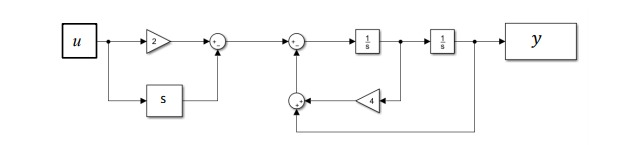
\includegraphics[width=\textwidth]{simulink}
\end{figure}\newpage
Notiamo subito che esso è equivalente a:
\begin{figure}[h]
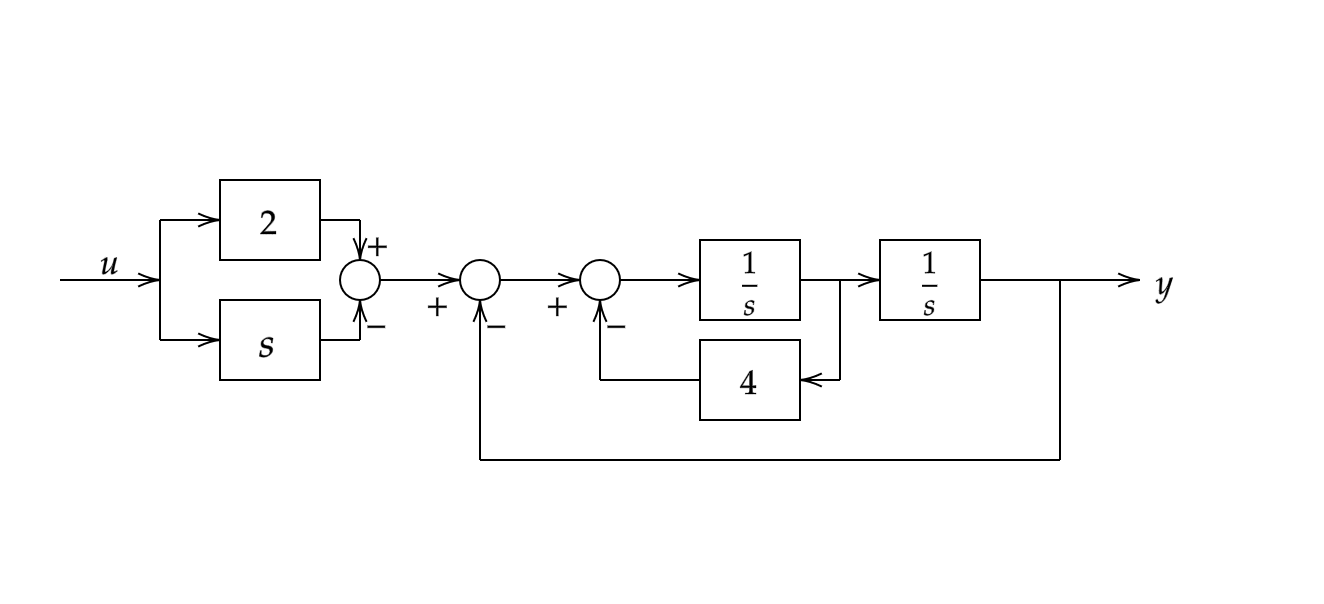
\includegraphics[width=\textwidth]{simusemp}
\end{figure}\newline
Che è equivalente a scrivere:
\[
\left(2\|s\right)\cdot \left(\left(\left(\frac{1}{s} \space \: \retroneg \:4\right)\cdot \frac{1}{s}\right)\retroneg\right)
\]
Che se svolto propriamente ci dà:
\[
G(s)=\frac{2-s}{s^2+4s+1}
\]
%=== firme ============================================================================
\vfill
\begin{flushright}
Luca Maci\\
Luca Paparo\\
Marco Poggi\\
Jacopo Stringara\\
Giulio Venturini
\end{flushright}
%=== fine documento ===================================================================
\end{document}
%=== Note =============================================================================

















